%% ****** Start of file aiptemplate.tex ****** %
%%
%%   This file is part of the files in the distribution of AIP substyles for REVTeX4.
%%   Version 4.1 of 9 October 2009.
%%
%
% This is a template for producing documents for use with 
% the REVTEX 4.1 document class and the AIP substyles.
% 
% Copy this file to another name and then work on that file.
% That way, you always have this original template file to use.

%\documentclass[aip,graphicx]{revtex4-1}
%\documentclass[aip,reprint]{revtex4-1}

%\usepackage{graphicx}

%\draft % marks overfull lines with a black rule on the right
%\documentclass[pre,aps,floatfix,authordate1-4,twocolumn]{revtex4-1}
%\documentclass[pre,aps,floatfix,authordate1-4]{revtex4-1}

\documentclass[aps,prl,superscriptaddress,twocolumn]{revtex4}



%\documentclass[aps,prl,preprint,groupedaddress]{revtex4}

\usepackage{rotating} 
\usepackage{times}
\usepackage{graphicx}
\usepackage{setspace}
\usepackage{amsmath}
\usepackage[obeyFinal]{easy-todo}
\begin{document}

% Use the \preprint command to place your local institutional report number 
% on the title page in preprint mode.
% Multiple \preprint commands are allowed.
%\preprint{}

\title{Atomistic resolution structure and dynamics of lipid bilayers in simulations and experiments} %Title of paper

% repeat the \author .. \affiliation  etc. as needed
% \email, \thanks, \homepage, \altaffiliation all apply to the current author.
% Explanatory text should go in the []'s, 
% actual e-mail address or url should go in the {}'s for \email and \homepage.
% Please use the appropriate macro for the type of information

% \affiliation command applies to all authors since the last \affiliation command. 
% The \affiliation command should follow the other information.

\author{O. H. Samuli Ollila}
\email[]{samuli.ollila@aalto.fi}
%\homepage[]{Your web page}
%\thanks{}
%\altaffiliation{}
\affiliation{Aalto University}


% Collaboration name, if desired (requires use of superscriptaddress option in \documentclass). 
% \noaffiliation is required (may also be used with the \author command).
%\collaboration{}
%\noaffiliation

\date{\today}

\begin{abstract}
% insert abstract here
Abstract.
\end{abstract}

%\pacs{}% insert suggested PACS numbers in braces on next line

\maketitle %\maketitle must follow title, authors, abstract and \pacs

% Body of paper goes here. Use proper sectioning commands. 
% References should be done using the \cite, \ref, and \label commands


%\label{}
\section{Introduction}
\todo{Samuli: Add citations to the introduction}
Atomistic resolution molecular dynamics simulations of lipid bilayers are nowdays
widely used technique to seek answer to various research questions.
Typically interactions between other biological molecules (e.g. proteins, drugs, ions etc.)
and lipids are studied but sometimes also lipid properties are directly under interest.
The questions are often biologically motivated and the atomistic resolutions simulations
gives very detailed information which is experimentally unattainable.

When simulations are used in this kind of studies, it is necessary to understand
the limitations of the method and also the accuracy of the used model.
In the pioneering atomistic resolution lipid bilayer simulations the quality of
the simulation respect to reality was measured mainly by comparing the 
acyl chain order parameters and area per molecule between experiments and
simulations. Especially some simulation models repruced these amazingly well
which led to the wide usage of these models.

Despite of the success of the models to reproduce the acyl chain properties and
molecular density more or less correctly, already early days it was pointed out
by comparing simulations to various experiments
that the glycerol backbone and choline headgroup order structure may not have been 
correctly described. However, at the time simulations were very short compared
to currently accessible timescles and it was not clear if the molecules had
time to sample all the states the model would predict. Also the method to 
quantitatively measure atomistic resolution molecular dynamics and compare to
simulations was not available, thus the real sampling timescales were not known.
For these reasons the estimates of the quality of headgroup were inconclusive on
the early days of molecular dynamics simulations of lipid bilayers and
the issue has gained more attention only very recently.

While the C-H bond order parameters for all hydrocarbon segments are yet the
core parameter to quantify the lipid model quality, the area per molecule 
is quite generally replaced with form factor.
The main reason is that the area per molecule is calculated from the scattering
data using a model (set of assumptions). Thus, when this value is compared to
the value from simulations, the simulations are not compared directly to experiments
but to a value which comes from another model (set of assumptions to calculate the
area per molecule). For this reason the area per molecule is nowdays replaced
by comparison between form factor from simulations and x-ray or neutron scattering.

In this review we discuss the current state of the art methods to compare the 
atomistic resolution lipid structure and dynamics in simulations to the experiments. 
The C-H bond order parameters measured with NMR and form factors measured
with x-ray or neutron scattering are discussed for structural comparison,
and spin lattice relaxation rates for the comparison of dynamics.
The main advantages of these parameters are that
the experimental techiques are non-invansive, they are measured from multilamellar phase 
which is practically always present in simulations as well due to periodic boundary conditions
and that the compared quantity (order parameter, spin lattice relaxation and form factor) is achieved from 
the actual experimental data in a robust way. The experimental results from these
experimental techniques are also highly reproducible and the measured timescales
are appropriate for the comparison to simulations. Also several other experimental
parameters and techniques are used to quantify the simulation quality, however,
none of these is as robust as order parameters, spin relaxation rates or form factor. The most
commonly used other techniques are shortly discussed in the end of the review.

In this review we focus on phosphatidylcholine (PC) lipids which has been
in the focus of fundamental structural lipid studies for several decades now. However, there is a lot
data available and the basis of our approach applies to other lipid types as well~\cite{??}.

\section{C-H bond order parameters as atomistic resolution structural measure}

\todo{This is the first sketch of this section. It is composed from the content in the blog
and from the things which came into my mind. A lot of references should be added, the text should polished,
things should be added and checked and figures should be improved. However, the main strucutre and idea of the section should be visible.}

%\noindent {\bf Here will be described:}\\[0.1cm]

%\noindent How are the order parameters measured.\\
%What is the primary experimental observable. \\
%How accurate are the experimental results. \\
%How order parameter is calculated from simulations. \\
%How accurate are the order parameters from simulations. \\
%What can be learned about the structure when comparing order parameters between experiments and simulations \\[0.5 cm]

\subsection{Definition and properties of C-H bond order parameter}\label{OPdefinition}
In lipid bilayer systems the order parameter of a hydrocarbon C--H vector is typically defined as 
\begin{equation}\label{orderP}
S_{{\rm CH}}=\frac{1}{2}\langle 3 \cos^2 \theta-1 \rangle,
\end{equation} 
where the angle brackets denote an ensemble average over the sampled conformations, and $\theta$ is the 
angle between the C--H bond and the membrane normal.
The numerical values of order parameters vary between $-\frac{1}{2} < S_{{\rm CH}} < +1$
depending on the sampled $\theta$ distribution.
The definition is motivated by its connection to the dipolar and quadrupolar splitting measured with
$^1$H-$^{13}$C and $^2$H NMR techniques, respectively. The functional form comes from 
the fundamental theory of interactions between spin systems which gives a connection between 
average molecules orientations and NMR measurables~\cite{abragam}. 

If the sampled distribution of $\theta$ for a C--H bond are known, the order parameter
can be straighfowardly calculated from Eq. \ref{orderP}. However, the sampled $\theta$ 
distribtions cannot be uniquely determined from the known order parameter. Thus the experimental
order parameter values gives a set of conditions which structural molecular model 
(more specifically the C--H bond vectors of the model) has to fulfill
but the experimental order parameters alone cannot be used to uniquely 
resolve the structure. The same applies practically to all
experimental parameters used in biomolecular structure determination. 

Atomistic resolution molecular dynamic simulations naturally produces the
sampled structures from which the $\theta$ distributions can be calculated and
used in Eq.~\ref{orderP} to calculate the order parameters.
The sampled structures in the simulation can considered to be realistic
only if the experimental order parameters are reproduced.
If this is the case, the simulation can be then considered 
as an atomistic resolution interpretation of experimental order parameters.
Before MD simulations were feasible for such usage, other models have been used for this interpretation~\cite{??}.
It is important to note, however, that the sampled structures which reproduce the order parameters are not 
necessarily the correct ones since, in principle, several structural models can produce the same order parameters. 
Significant advance of the MD models compared to the traditional models is that the same MD 
structures can be straightforwardly compared to other experimental observables in addition to order parameters, 
like $^{31}$P chemical shift anisotropy~\cite{chowdhary13}, $^{31}$P-$^{13}$C dipolar couplings~\cite{prakash10}
and scattering data~\cite{??}. This will significantly reduce the 
possibility of getting unrealistic structures reproducing correct order parameters.

The probability for unrealistic structures with correct order order parameters is further reduced by
the detailed and accurate experimental data available for order parameters.
Order parameters are known with high quantitative accuracy for each C-H bond present in the lipid molecule
for several lipid types~\cite{??}. The absolute values of order parameters can be measured two independent
techniques by using either $^2$H NMR~\cite{seelig77c} or $^1$H-$^{13}$C NMR~\cite{hong95a,gross97,dvinskikh05a,ferreira13} and
the sign can be measured with two different $^1$H-$^{13}$C NMR techniques~\cite{hong95a,hong95b,gross97}.
It is also possible that two hydrogen bonds in the same carbon has different order parameters ({\it forking})
which can be detected with both $^2$H NMR~\cite{??} and $^1$H-$^{13}$C NMR~\cite{??} techniques.
As a result, for example for POPC lipid molecule in lipid bilayer there is ? order parameter numbers
known experimentally and a structural model for this lipid should reproduce all of these.
If some the order parameters are not reproduced, it is easy to detect the weak parts of the model
since a single order parameter is very local quantity depending only on the position of two atoms (C-H pair).
This is an advance over several other accurately measured NMR quantities, 
like $^{31}$P chemical shift anisotropy~\cite{chowdhary13} and $^{31}$P-$^{13}$C dipolar couplings~\cite{prakash10}
which depend on the position of several atoms, thus in the case of disagreement, it is more difficult 
to pinpoint the problems in the model.

%if discprepancy is found in order parameter related to certain bond it is known that the model has problems
%in the orientation of this specific bond. This gives order parameters a significant advance over, e.g. other
%accurate NMR obervables like ??. These can be also used to quantify the structural quality, however, in the
%case of disagreement the problem points in the model are more difficult to localize.


%In sections~\ref{??} and~\ref{??} we review the most relevant experimental and molecular dynamics simulation aspects related to the usage of
%order parameters in order to interpret the atomistic resolution structure of lipid bilayers. In section~\ref{??} we
%discuss the connection between structure and order parameters.





 

\subsection{Order parameters from $^2$H NMR experiments}

The absolute values of order parameters are connected to the quadrupolar splitting $\Delta \nu_Q$ ($^2$H NMR) 
measured in $^2$H NMR experiments through the equation 
\begin{equation}\label{HNMRop}
|S_{{\rm CD}}|=\frac{4}{3} \frac{h}{e^2qQ} \Delta \nu_{{\rm Q}}, 
\end{equation}
where $e$ is the elementary charge, $Q$ is the deuteron quadrupole moment and $h$ is the Planck's constant. 
The parameter $q$ is related to the largest electric field gradient and in practise its value is not known; 
therefore the static quadrupolar coupling constant $\frac{e^2qQ}{h}$ is defined, and its value measured for 
different compounds in their solid state ($\Delta \nu_Q$ measurement from the system where order parameter is known to be 1). 
In C-D order parameter measurements for lipids, it is typical to 
use the value measured for different alkenes, $\frac{e^2qQ}{h}$=170 kHz. The relation between order parameters 
and quadrupolar splittings then becomes $S_{{\rm CD}}=0.00784 \times \Delta \nu_{{\rm Q}}$.
This relation is useful as many publications report only the quadrupolar splittings. For a review and more accurate description see the work of Seelig~\cite{seelig77c}.

\subsection{Order parameters from $^{13}$C NMR experiments}

To determine order parameter with $^1$H-$^{13}$C NMR experiments, the dipolar splitting $\Delta \nu_\mathrm{CH}$  is measured. This is then related to
the effective dipolar coupling $d_\mathrm{CH}$ through a scaling factor depending on the pulse sequence used in the 
experiment~\cite{hong95a,gross97,dvinskikh05a,ferreira13}. The effective dipolar coupling $d_{{\rm CH}}$ is 
connected to the absolute value of order parameter through equation
\begin{equation}\label{CNMRop}
|S_{{\rm CH}}|=(\frac{D_{{\rm max}}}{2\pi})^{-1}d_\mathrm{CH},
\end{equation}
where $D_{{\rm max}} = \frac{\hbar \mu_0 \gamma_h \gamma_c}{4\pi\langle r_\mathrm{CH}^3 \rangle}$. 
$r_{{\rm CH}}$ is the C-H distance, $\mu_0$ is the vacuum permittivity, and $\gamma_h$ and $\gamma_c$ are 
the gyromagnetic constants for $^1$H and $^{13}$C nuclei. In contrast to Eq.~\ref{HNMRop}, all the parameters in 
Eq.~\ref{CNMRop} are in principle known. However, for the internuclear distance only the average $⟨r_{{\rm CH}}⟩$ 
is known, not the third moment $⟨r^3_{{\rm CH}}⟩$. For this reason values between 20.2-22.7 kHz are used for
$\frac{D_{{\rm max}}}{2\pi}$ depending on the original authors~\cite{hong95a,gross97,dvinskikh05a,becker06,ferreira13,ferreira15}.

\subsection{Quantitative accuracy of experimental order parameter values}

It must be stressed that $^2$H NMR and $^{13}$C NMR are fully independent experiments since the deuterium quadrupolar splitting $\Delta \nu_Q$
and the dipolar splitting $d_{{\rm CH}}$ are different physical observables. In addition, the prefactors connecting the observables to the order 
parameter (Eqs.~\ref{HNMRop} and~\ref{CNMRop}) are independently measured. Further independent experiments are performed With $^{13}$C NMR 
by measuring the $^1$H-$^{13}$C dipolar couplings using different pulse sequences~\cite{hong95a,gross97,dvinskikh05a,ferreira13} when the connection
between dipolar splitting $d_{{\rm CH}}$ and effective dipolar coupling $d_\mathrm{CH}$ is different.

The measurements of quadrupole $\Delta \nu_Q$ and dipolar $d_{{\rm CH}}$ splittings are relatively accurate, especially for quadrupolar splitting.
\todo{How accurate exactly?} 
Thus the quantitative accuracy of measured order parameters is mainly determined by the  
prefactors connecting the measured splittings to the order parameters (Eqs.~\ref{HNMRop} and~\ref{CNMRop}). 
Since the prefactors are independently determined for the $^2$H and $^{13}$C NMR measurements,
the quantitative accuracy is best estimated by comparing the independtly measured order parameter values.

The comparisons between order parameters measured with $^2$H NMR and $^{13}$C NMR by several authors
shows very good agreement~\cite{gross97,dvinskikh05a,ferreira13, botan15}.
Botan et al. collected literature values for PC lipid choline headgroup and glycerol backbone order parameters 
and concluded that order parameters would be known with the accuracy of $\pm$0.02 for these segments in purified PC lipid bilayer samples~\cite{botan15}
which agrees with the estimate of Gross et al~\cite{gross97}. 
The lower order parameter reported in some studies~\cite{hong95a,hong95b,warschawski05} were suggested to arise from lower experimental accuracy.
The values collected by Botan et al. and the suggested sweet spots where choline and glycerol backbone order parameters should fall in the 
simulation models are shown in Fig.~\ref{allOPs} A).
\begin{figure*}[]
%  \centering
  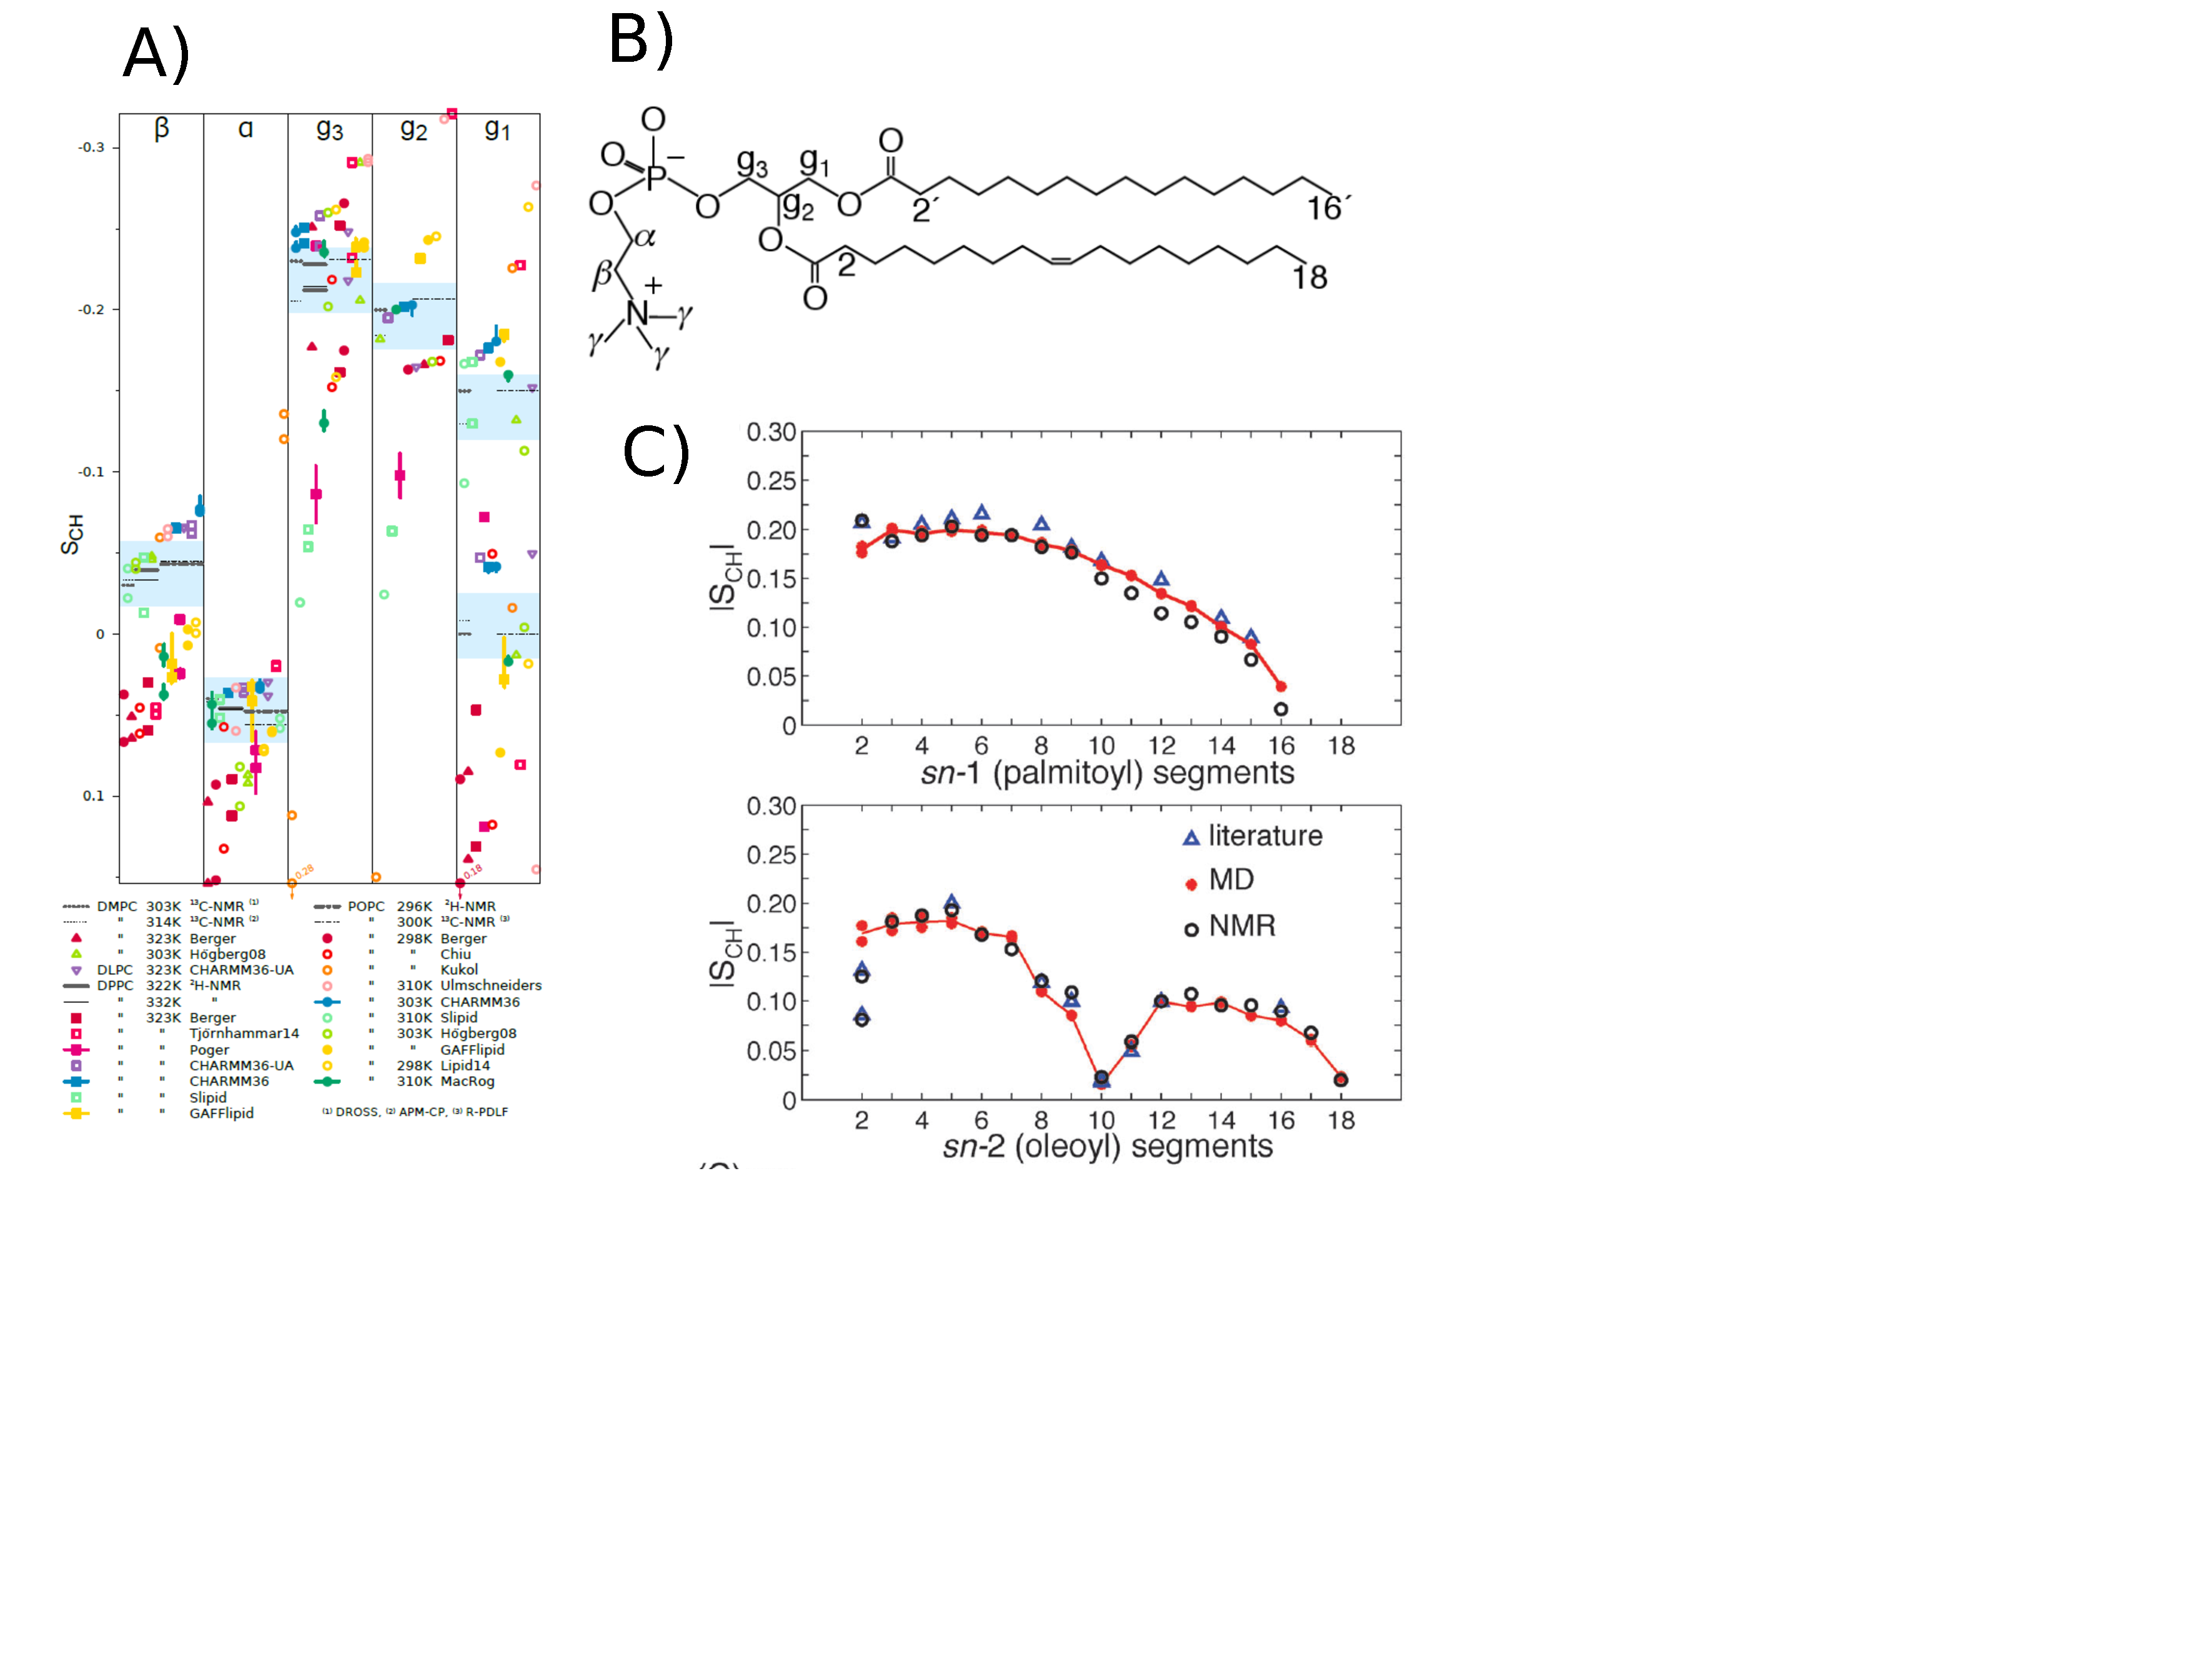
\includegraphics[width=17.2cm]{../Fig/allOPs.eps}
  \caption{\label{allOPs}
    A)  Order parameteres from simulations and experimental values from literature for glycerol and choline groups collected by Botan et al.~\cite{botan15}.
    The experimental values were taken from the following publications:
    DMPC 303~K from \cite{gross97},
    DMPC 314~K from \cite{dvinskikh05a},
    DPPC 322~K from \cite{gally75},
    DPPC 323~K from \cite{akutsu81},
    POPC 296~K from \cite{bechinger91}, and
    POPC 300~K from \cite{ferreira13}.
    The vertical bars shown for some of the computational values are not error bars, but demonstrate that for 
    these systems we had at least two data sets (see Table 1 in Botan et al.~\cite{botan15});
    the ends of the bars mark the extreme values from the sets, and the dot marks their measurement-time-weighted average. 
    The interactive version of this figure is available at  https://plot.ly/$\sim$HubertSantuz/72/lipid-force-field-comparison/.
    B) Chemical structure of 1-palmitoyl-2-oleoylphosphatidylcholine (POPC).
    C) Picture adapted from~\cite{ferreira13}.
    Order parameter magnitude $|S_{{\rm CH}}|$ vs. carbon segment number for the
    sn-1 and sn-2 acyl chains of POPC (A and B respectively). Data from fully hydrated POPC at
    300 K obtained with $^1$H–$^{13}$C solid-state NMR (black dots)~\cite{ferreira13} and MD simulations
    (red dots)~\cite{ferreira13}, as well as data from 2H NMR (blue triangles) (sn-1~\cite{seelig78} and
    sn-2~\cite{seelig78,perly85} at 300 K).
  }
\end{figure*}

Acyl chain order parameters from different techniques are compared in Table 1 by Gross et al.~\cite{gross97}, 
Dvinskikh et al.~\cite{dvinskikh05a} and Ferreira et al.~\cite{ferreira13}. The comparison by Ferreira et al.~\cite{ferreira13} 
is also shown in Fig.~\ref{allOPs} C). Generally good agreement between different methods is seen also for
acyl chain order parameters, however, for some segments the 0.02 accuracy might not be achieved.
\todo{Maybe specify to which ones?}.

%In conclusion, comparing the order parameters measured with different techniques based on different physical interactions 
%the accuracy of the prefactors can be estimated. Since the order parameters from different techniques are 
%almost always within $\pm$0.02 this can be considered to be the quantitative accuracy of the measurements.


\subsection{Qualitative accuracy of experimental order parameter values}

When order parameters are measured as function of changing condition (e.g. temperature, hydration level, ion concentration, etc.), 
the prefactors connecting the order parameter and the experimentally measured couplings can be considered 
to be unchanged. Therefore, accuracy of the measured change is determined by the accuracy of the splitting measurement
in contrast to the previous section. Here we refer to this as a qualitative accuracy. Due to the high resolution of
splitting measurements, especially in $ 2$H NMR, the qualitative accuracy is much higher than the
quantitative accuracy discussed in previous section.

The high qualitative accuracy of $ 2$H NMR experiments is exemplified in Fig. \ref{??} by using the
the classical experiment by Akutsu and Seelig~\cite{akutsu81}, where the effect of different ions on 
the quadrupolar splittings of choline headgroup $\alpha$ and $\beta$ segments was measured, 
\footnote{These changes were later shown to be consistent with the addition of different charges into the bilayer, and the electrometer 
concept was introduced to measure the amount of charge incorporated in the bilayer interface~\cite{scherer89}.}
see Fig.~\ref{QUADsplitIONeffect}. 
The effects of different ions on the quadrupole splittings are clearly differentiable with the experimental 
accuracy in Fig.~\ref{QUADsplitIONeffect} A). However, when transformed to the order parameter units, 
these changes correspond only changes below 0.03 units for $\beta$ and 0.05 for $\alpha$ as shown in 
Fig.~\ref{QUADsplitIONeffect} B). 
\begin{figure*}[]
%  \centering
  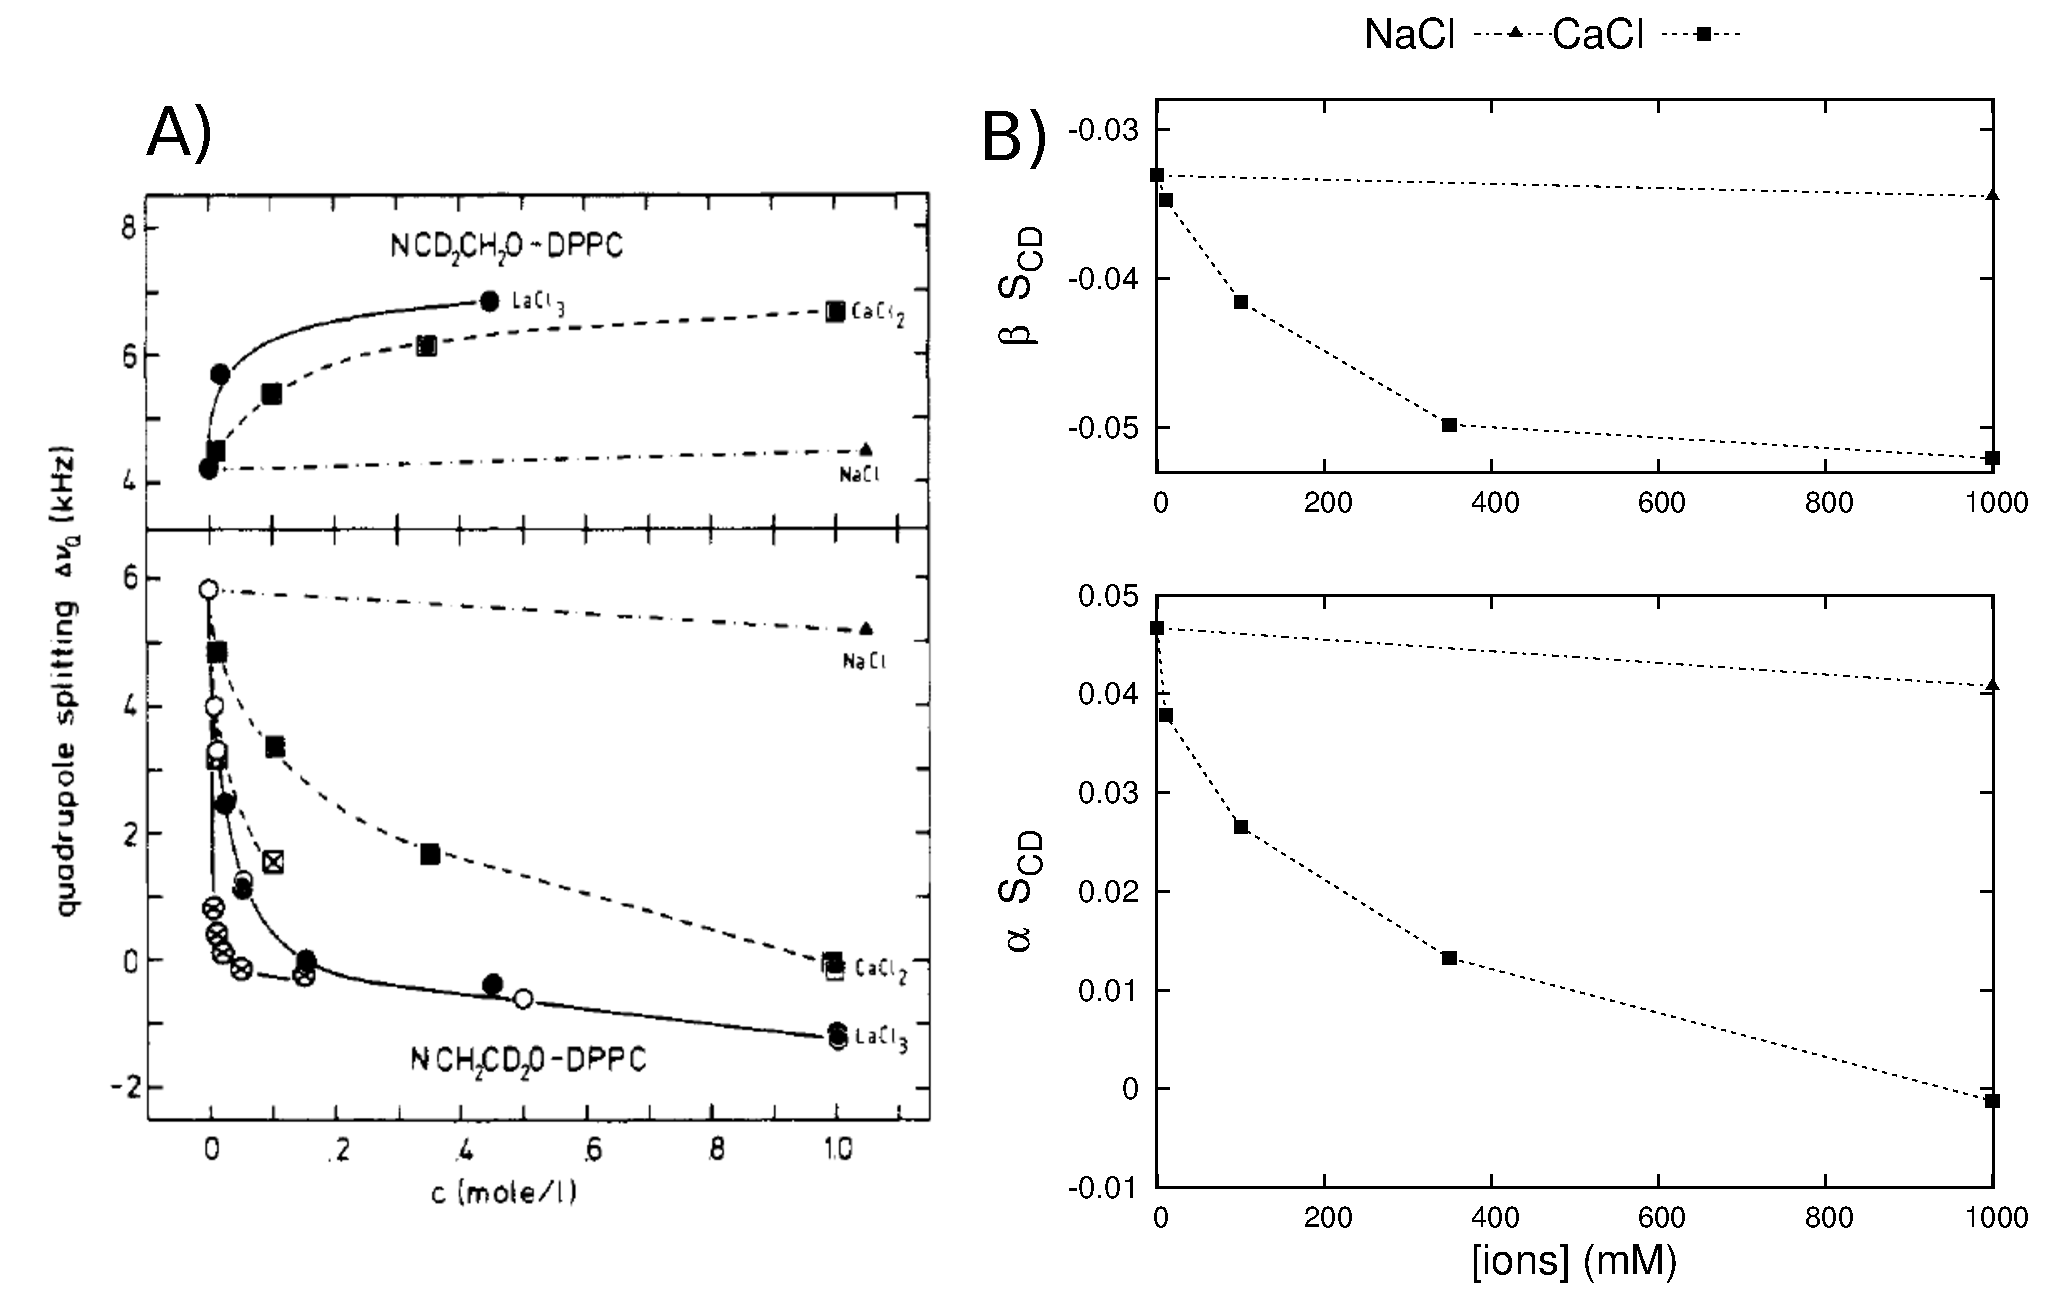
\includegraphics[width=17.2cm]{../Fig/QPandOPwithIONS.eps}
  \caption{\label{opIONeffect}
    A) Quadrupolar splittings as function of different ion concetrations measured by Akutsu and Seelig with $^2$H NMR~\cite{akutsu81}. 
    B) The data from A) translated to order parameters ($S_{{\rm CD}}=0.00784 \times \Delta \nu_{{\rm Q}}$). Also the sign of $\beta$ order parameter is put negative according
    to more recent experiments~\cite{??} (see also Ref.~\cite{botan15} and Section~\ref{??}).
  } 
\end{figure*}

%The resolution of $^{13}$C NMR experiment depends somewhat on the pulse sequence used. 
As another example of the high qualitative accuracy of order parameter experiments, the measured order parameters
for $\beta$ and $\alpha$ carbons as a function of hydration level for different PC lipids are shown in 
Fig.~\ref{opDEHYDeffect}. Quantitative numbers from different experiments show slight variation between
different temperatures and lipid compositions. However, in all experiments the
order parameters increase with decreasing hydration.
\footnote{This increase is related to the P-N vector tilting more parallel to the membrane plane \cite{botan15}
which is in agreement with electrometer concept suggesting that penetrating charge has opposite 
effect on headgroup tilt leading to decrease of order parameters \cite{scherer89,ionpaper}.}
The smallest order parameter change is only slightly above 0.01 units, measured by Dvinskikh et al. 
with $ 13$C NMR~\cite{dvinskikh05b}, demonstrating that high qualitative accuracy can be
also achieved with $ 13$C NMR. 
\begin{figure}[]
%  \centering
  \includegraphics[width=8.6cm]{../Fig/OrderParameterDEHYDexp.eps}
\newline
  \caption{\label{opDEHYDeffect}
    Dehydration changes on $\alpha$ and $\beta$ order parameters measured with different methods. 
    The data taken from Dvinskikh et al.~\cite{dvinskikh05b}, Ulrich et al.~\cite{ulrich94} and Bechinger et al.~\cite{bechinger91}
    Also the sign of $\beta$ order parameter is put negative according
    to more recent experiments~\cite{??} (see also Ref.~\cite{botan15} and Section~\ref{??}).
  } 
\end{figure}

In conclusion, the experimental qualitative accuracy order parameter measurements is very high.
It is much higher than the accuracy achieved with state of the art MD simulations.
Thus, the accuracy order parameter change comparison between simulations and experiments is
limited by the simulation accuracy, not experimental. 

On the other hand, it should be noted that since even very small splitting changes can 
be detected experimentally one should always connect these to the changes in real molecules
to avoid overinterpretation. For example, it has been measured that cholesterol induces 
a measurable change in ? quadrupolar splitting which is ? \cite{??}. This may tempt to conclude that
cholesterol affects to the choline structure, however, this quadrupolar splitting corresponds
? unit change in the order parameter which indicates almost negligible conformational change \cite{botan15}.


\subsection{Signs of order parameters}

While only the absolute values of order parameters are accessible with $^2$H NMR, two different 
$^1$H-$^{13}$C NMR techniques allow also the measurement of the sign: 
first Hong et al. first measured order parameter signs for eggPC~\cite{hong95a} and DMPC~\cite{hong95b}; 
then later Gross et al. used a different NMR technique to measure signs for DMPC~\cite{gross97}. 
All the experiments report negative order parameters for almost all the segments, only $\alpha$ and $\gamma$ are positive.

Furthermore, the signs~\cite{hong95a,hong95b,gross97}  and magnitudes~\cite{gally81,ferreira13,botan15} of choline headgroup 
and glycerol backbone order parameters are practically unaffected by the acyl tail contents of the bilayers. 
Thus, it can be fairly assumed that the order parameter signs for these segments are the same in all PC lipids in bilayer. 
On the other hand, the positive signs for g$_1$, g$_3$ and C$_2$ has been reported by Aussenac et al.~\cite{aussenac03} 
which has led to some confusion in comparison between simulations and experiments~\cite{hogberg08}. 
However, these signs are not directly measured but extracted from the model used to interpret 
$^2$H NMR order parameters from DMPC bicelles. Thus, it is reasonable conclude that 
order parameters are negative for all segments except for $\alpha$ and $\gamma$, as 
directly measured with $^1$H-$^{13}$C NMR~\cite{hong95a,hong95b,gross97}.

Even though the sign was not measurable with $^2$H NMR, the sign was believed to be negative for acyl chains because $\theta$ was expected to fluctuate 
around 90$^o$ leading to negative order parameters~\cite{seelig77c}. This was later confirmed by using $^{13}$C NMR measurements~\cite{hong95a}. 
Also MD simulations always produce negative order parameters for acyl chains.

%In conclusion, it seems reasonable to assume that the signs measured with $^{13}$C NMR methods~\cite{hong95a,hong95b,gross97}
%can be used for all PC lipids in bilayer, i.e. the signs for almost all the carbons are negative, only  $\alpha$ and $\gamma$ are positive.

Typically when the response of order parameters to varying conditions (ions, dehydration and cholesterol) is measured, only the absolute 
values are reported~\cite{akutsu81,altenbach84,bechinger91,ulrich94,dvinskikh05b,ferreira13}. Where clear responses are observed, 
like with multivalent ions~\cite{akutsu81,altenbach84} and dehydration~\cite{bechinger91,ulrich94,dvinskikh05b}, the experiments are done by gradually 
changing the conditions and the order parameter response is systematic, see Figs.~\ref{opIONeffect} and~\ref{opDEHYDeffect}. 
Thus, it is reasonable to assume that also the signs are not suddenly changing. However, it seems that the sign of 
the $\alpha$ carbon order parameter does change in response to a large amount of bound charge, such as multivalent ions. In this case, 
the absolute value of the order parameter first decreases to zero and then starts to increase again~\cite{altenbach84,seelig87}, 
as seen from the nicely illustrated spectra shown Fig.~\ref{qsCACLeffect} by Altenbach et al.~\cite{altenbach84}.
\begin{figure}[]
%  \centering
  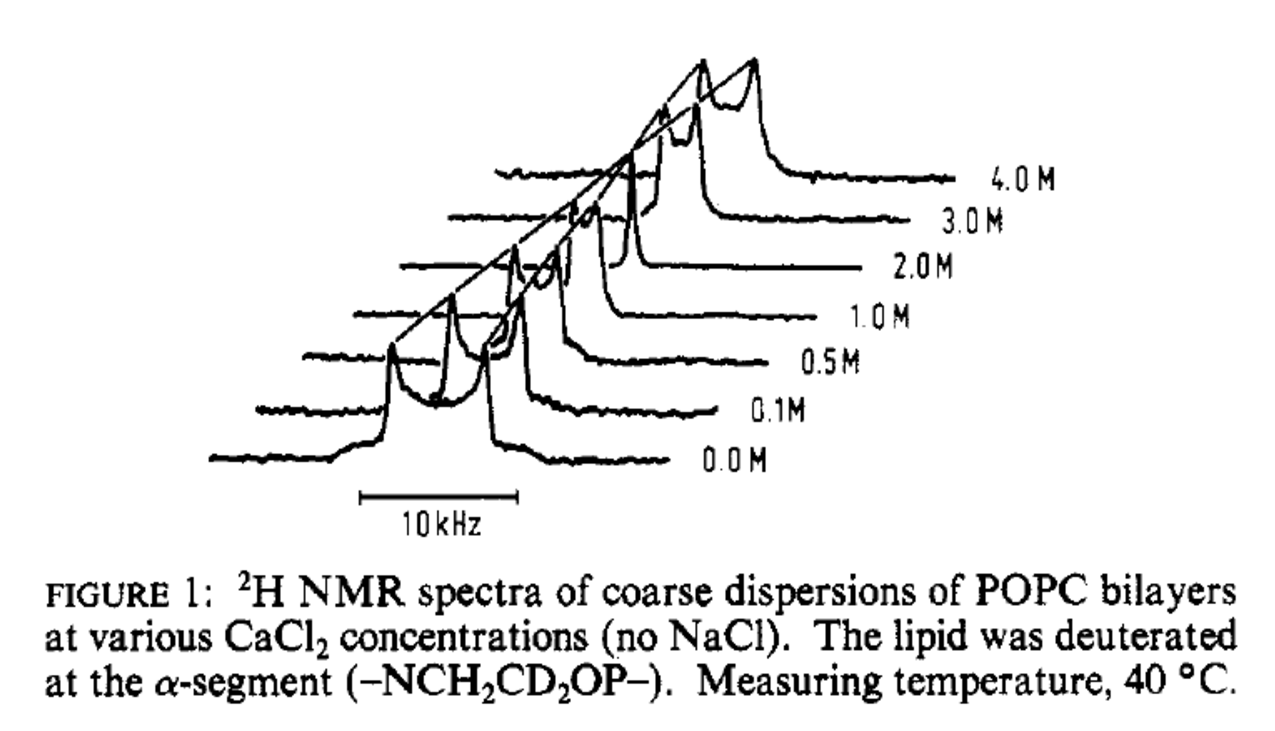
\includegraphics[width=8.6cm]{../Fig/QUADsplitCACLeffect.eps}
\newline
  \caption{\label{qsCACLeffect}
    Quadrupolar splitting $\Delta \nu_Q$ of $\alpha$ of POPC as a function of CaCl$_2$ concentration, related to the order parameter as $S_{{\rm CD}}=0.00784 \times \Delta \nu_Q$. 
    We know nowadays that the order parameter of $\alpha$ in the absense of CaCl$_2$ is positive~\cite{hong95a,hong95b,gross97}.
    Thus, the most obvious interpertation for the result is that the $\alpha$ order parameter decreases to zero when CaCl$_2$ concentration reaches 2.0M, and 
    above these concentrations becomes increasingly negative with further addition of CaCl$_2$. Reprinted with permission from Altenbach and Seelig, Biochemistry, 23, 3913 (1984). Copyright 1984 American Chemical Society.    
  } 
\end{figure}



\subsection{Forking of order parameters}

It is possible that the CH$_2$ segment is sampling such orientations that the order parameters
for different hydrogens in the same carbon have different values. We call this phenomena as 
{\it forking}, as done also previously to avoid confusion with splittings measured with NMR.
The forking is detected with both $^2$H NMR~\cite{seelig75,seelig78,engel81,gally81} and 
$^1$H-$^{13}$C NMR techniques~\cite{??} as two different quadrupolar or dipolar splitting values,
respectively, related to the same CH$_2$ segment.

The forking is observed for g$_1$, g$_3$, and  C$_2$ carbon in the \textit{sn}-2 chain segments in
a fluid PC lipid bilayer, for other CH$_2$ segments the equal order parameters are observed for 
both hydrogens are equal~\cite{seelig74,seelig77,seelig78,gally81,ferreira13,??}.
The forking has been studied in detail with $^2$H NMR techniques by separately deuterating the 
R or S position in CH$_2$ segment to assign order parameters to correct hydrogens \cite{gally81}.
\todo{Has this been done for the C$_2$ carbon in the \textit{sn}-2 chain?}

$^2$H NMR studies also show that the forking really arises from differently sampled orientations 
of the two C--H bonds, not from two separate populations of lipid conformations~\cite{engel81,gally81}.
This means that realistic atomistic resolution molecular models has to reproduce the forking 
correctly. Thus, the simulated order parameters has to be calculated separately for each hydrogen
by taking into account the isomeric position for the structural comparison to the experimentals.
Recent work by Botan et al. shows that several simulation models has problems in this respect \cite{botan15}
(see also Fig. \ref{??}). 


\subsection{Order parameter values in the literature}
For $^2H$ NMR measurements the CH$_2$ segments has to be labeled with deuterium.
This can be done specifically for a certain segment or for the several segments
simultaneously \cite{??}. In the first case, it is known that the measured
order parameter (quadrupolar splitting) is related to the labeled segment.
In the latter case several order parameters (quadrupolar splittings) are
measured which arise from all the labeled segments, however, it is not known 
which order parameter belongs to which segment. Majority of the $^2H$ NMR data
in the literature is measured from samples with perdeuterated acyl chain \cite{leftin11}
since the synthesis of specifically deuterated lipids is complicated \cite{??} and they are expensive.
From this kind of data alone one cannot know which order parameter is assigned
to which CH$_2$ segment. On the other hand, also order parameter data from specifically 
deuterated lipids are available from several lipid types in various 
conditions \cite{seelig74,seelig75,seelig77,seelig78,gally81}.

Specific labeling is not needed for order parameter measurement with $^{13}$C NMR due the 
natural abundance of $ {13}$C, however it could be used to enhance the signal for specific 
segment under interest \cite{??}. Order parameter measurements with $^{13}$C NMR are
2D experiments, the chemical shift being in the first dimension and dipolar coupling 
in the second \cite{??}. The chemical shift depends on the local chemical environment and 
is different for each carbon segment. In the second dimension the dipolar coupling
(order parameter) corresponding each chemical shift value is measured, and its value 
can be connected, in principle, to each carbon segment by using the chemical shift value.  
In practise, challenges occur in the acyl chain region where chemical shift values 
of different segments are very close to each others \cite{??}. This issue has been
addressed by filtering the spectra by using partially deuterated lipids \cite{ferreira13}
and using data from simulations and specifically deuterated experiments to help in 
the assigment \cite{ferreira13,??}. It should be noted that the overlapping spectra 
is a challenge only for acyl chain regions with several similar segments. On the other hand, 
the order parameters for hydrocarbon segments in choline, glycerol backbone, close to the 
double bonds, and in the beginning and the end of acyl chains can be straighforwardly 
measured from the natural abundance lipid samples. 

The order parameters are typically measured from multilamellar samples which are good for comparison to MD 
simulations since it a nearest experimental correspondence for a simulation box with periodic boundary conditions. 
In this work we do not discuss order parameters can be measured also from other type of samples, 
e.g. bicelles~\cite{aussenac03,raffard00,sanders92}, or indirect measurements by using, e.g. relaxation
data~\cite{??} since their comparison to simulations is less straightforward.  

The available experimental data for order parameters is reviewed
quite recently~\cite{leftin11,marsh13}. These reviews are comprehensive especially for 
acyl chains in pure lipid bilayer samples. In addition to this, there is significant
amount of order parameter data for glycerol backbone and headgroup segments \cite{botan15}, and
also data as a function of changing conditions for all lipid segments \cite{??}.
The amount of data, especially from $^{13}$C NMR, has been also increasing lately~\cite{ferreira13,leftin??,??}.
Especially the order parameter data of headgroup responses to varying conditions 
has a lot of unused pontential since it can used to measure, e.g. ion partitioning to lipid
bilayer \cite{??,ionpaper} and lipid protein interactions \cite{??}. Simultaneously, it
gives accurate experimental parameters which can be directly compared to MD simulations \cite{botan15,iopaper}.



\subsection{Order parameters from simulations}
In atomistic resolution molecular dynamics simulations molecules are sampling the defined ensemble
according to the used simulation parameters and the coordinates of each atom as a function of time are saved
to the trajectory files. The coordinates in the trajectory file can be straighforwardly used to calculate 
order parameters directly from the definition in Eq.~\ref{orderP}. The average is taken over the molecules and time.

For simulations with united atom models without explicit hydrogen atoms~\cite{??}, the hydrogen positions 
can be generated post-simulationally from the positions of the heavy atoms and the known hydrocarbon geometries.
This can be done explicitly by creating a trajectory with added hydrogens~\cite{??}, or by using equations
which directly calculate order parameters from heavy atom positions~\cite{??}.
For C--H and C--H$_2$ segments without forking these two approaches gives essentially identical results
when applied correctly. However, the latter is valid only for the cases with no forking, i.e. order 
parameters are equal for both hydrogens attached to the same carbon. Since this is not known {\it a priori}
for the analyzed model, it is better to use the first approach with explicitly added hydrogens.

The difference in the forking analysis is most likely reason for different choline and glycerol
backbone order parameters reported in the literature for the same model~\cite{poger??,botan15}.
Also different order parameters from the same model for C-H bonds has been reported in literature~\cite{??,??}
which most likely arises from incorrect implementation of widely used version of {\it g\_order} program in the Gromacs package
for this segment. Also, the {\it g\_order} program prints -S$_{{\rm CH}}$ which is most likely the reason to
the reported positive order parameters for acyl chains in some studies~\cite{??}.
When these issues are taken into account, the order parameters from the same models reported in the
literature are generally in good agreement.

The statistical error estimates for order parameters in simulations are estimated by
using the error of the mean calculated averaging over time blocks~\cite{ollila07}, over independent 
simulations~\cite{poger12} and over different lipids~\cite{botain15}. The maximum error bars given by
all these approaches are $\sim \pm$0.01.

It was recently pointed out that the sampling of individual dihedral angles might be very
slow compared to the typical (100~ns) simulation timescales~\cite{vogel12}.
This result raises a question if typical simulation time scales are long enough to allow
the molecules to sample the full phase phase. On the other, another recent study showed
that the slowest rotational auto-correlation function observed (for g$_1$ segment) 
in the Berger model reached a plateau ($S_\mathrm{CH}^2$) after $\sim$200~ns
and its relaxation was significantly too slow compared to NMR relaxation experiments~\cite{ferreira15}. 
This indicates that if the typical simulation times are too short for the full sampling
of the structures, then the dynamics is unrealistically slow in the simulation model.


\subsection{Comparison between order parameters from simulations and experiments}

The acyl chain order parameters are commonly calculated and compared to experiments
in simulation studies. Practically all force field parametrization publications report these
as one of experimental parameters which the models are reproducing in good agreement \cite{??}.
Indeed the agreement between simulations and experiments is almost always in strikingly good 
for acyl chain order parameters in pure lipid bilayers in full hydration \cite{??}, see also Fig \ref{??}.

Exception is the C$_2$ segment in {\it sn-2} chain in all PC lipids which is known
to have measurable forking and lower magnitudes compared to other order parameters in 
the beginning of the acyl chain \cite{??}. This important structural fingerprint is
related to the different conformations between carboxyl segments in the beginning of chains \cite{??}.
This feature is, however, not reproduced by several lipid models \cite{??} while other ones have been
more successfull \cite{??}.

In addition to the quantitatively good agreement in pure bilayers, the changes in 
acyl chain order parameters as a function of changing conditions are generally reasonable.
For example, experimentally observed increase of order parameters as a function of cholesterol 
concetration \cite{??} and with dehydration \cite{??} are reproduced in simulations \cite{??}. 
However, systematic and quantitative comparisons of these effects between experiments and simulations are rare.
Comparison between widely used model (Berger lipids \cite{??} and Höltje cholesterol model \cite{??}
\footnote{In this work CH$_2$/CH$_3$ groups in cholesterol were changed to LP$_2$/LP$_3$ groups to make it more consistent with the Berger
parameters. This is not usually done in the studies done with these model.})
for cholesterol containing lipid bilayer revealed that even though the acyl chain response is reasonable,
the simulation model cannot be considered to agree with experiments with 34\% and higher cholesterol concentrations.
CHARMM36 model has been shown to slightly underestimate the cholesterol ordering effect in DMPC bilayer \cite{??},
while Slipids and Lipid14 models show satisfactory agreement. Lipid14 is also compared to the same
extensive experimental data for POPC/cholesterol as Berge/Hötje model and the agreement is significantly better \cite{??}. 
Also the orientation of cholesterol itself is reasonable in all models \cite{??}, however, the cholesterol
acyl chain has some issues in Höltje model (too low order parameters) and in Lipid14 (significant forking) while
CHARMM36 reproduces experiments well \cite{??}. Despite of the problems the Höltje model 
is used to study the cholesterol acyl chain length effect on bilayer properties \cite{??}.  

The decrease of acyl chain order parameters due to the addition of double bonds is also 
generally reproduced by different simulation models \cite{??}. For oleyl chain in POPC 
with one {\it cis} double bond the
order parameters around double bonds are in almost perfect agreement with experiments
in many models \cite{??} (see also Fig. \ref{??}) but practically all models reproduce some
kind of decrease \cite{??}. Also the difference between {\it cis} and {\it trans} double bonds
can be reproduced in MD simulations \cite{??}.

In contrast to acyl chains, the order parameters for the glycerol backbone are not routinely
reported in simulation literature and when reported, the agreement with experiments is concluded to
be poor \cite{??} or good \cite{??} depending on the authors, not on the numbers reported.
This probably due to different estimations of the accuracy of experimental and simulated order parameters,
see also section \ref{??}.
The NMRLipids collaboration recently carefully compared glycerol backbone and choline order parameters  
from 12? different models to the experiments and concluded that none of the available models
reproduces these within experimental error, see Fig.~\ref{HGorderparameters}.
Also responses of glycerol backbone and choline order parameters to 
dehydration, cholesterol concetration and charge penetration were 
studied by the NMRLipids collaboration \cite{botan15,ionpaper}.
Despite of the incorrect structures in simulation models the experimentally measured choline order
parameter increase due to dehydration \cite{botan15} and decrease due to penetrating 
ions \cite{ionpaper} (see Fig. \ref{??}) were qualitatively reproduced. 
The comparison reveals, however, that the Na$ +$ penetration is significantly
overestimated by many models \cite{ionpaper}. 
Also the effect of cholesterol on glycerol backbone and choline was overestimated
by the Berger/Höltje model while CHARMM36 and MacRog performed better \cite{botan15}. 

In conclusion, the experimental order parameters for acyl chains and their changes are resonably
reproduced all state of the art lipid models (except for C$_2$ segment in {\it sn}-2).
However, all models have difficulties with varying severity to reproduce the glycerol backbone
and choline order parameters, and their changes.



\subsection{Interplay between simulations and NMR order parameters: Validation and interpretation}

As reviewed here, the order parameters can be measured with high accuracy for each hydrocarbon segment in lipid
in bilayer and the values are available in the literature for wide range of different lipids in different conditions.
Thus, the experimental order parameters give very detailed and local information about the orientations
sampled by each C--H bonds in the lipid bilayer system. The order parameters can 
be also calculated from MD simulations with high accuracy and compared to the experiments.
If the order parameters agree within experimental error, the simulated structures can considered as
an structural intepretation for order parameter experiments. On the other hand, if the agreement is not good, 
the simulation is sampling incorrect structures.

As discussed in the previous section, the order parameters for acyl chain region from MD simulations generally 
agree well with experiments (except for the C$_2$ segment in the {\it sn}-2 chain). Thus, the acyl chain structure 
is most likely realistic in simulations and they can used for structural interpretation for this region. 
This is a significant advancement to the traditional structural models build based on the 
fittings to the order paramters~\cite{??}. The dynamical visualization of simulation trajectory immediately 
reveals very dynamical nature of acyl chains, rapidly sampling large amount of different conformations 
(for dynamics see the Section~\ref{??}). These videos published by several authors in supplementary information~\cite{??}
gives significantly better intuitive understanding of dynamical nature of lipid bilayers compared to the static ones from 
traditional models. Since the lipid bilayers can be considered as a simplistic models for cell
membranes and other biological lipid layers, this understanding has significant impact on
biophysics and biochemistry. 

Also the order parameter changes with changing conditions are qualitatively reproduced in the acyl chain region, 
however the systematic quantitative comparison of changes is rare~\cite{??}.
The MD simulations have been especially useful to explain the origin of order parameter decrease
due to {\it cis} double bonds in the acyl chain~\cite{??}. The order parameter decrease might arise
from reduced order of the chain or from the changed average $\theta$ angle in Eq.~\ref{??}.
From NMR experiments alone it was impossible to judge which is the correct explanation for
the decreased order parameters due double bonds~\cite{??}. Several simulation studies by different
authors using different models has showed that the decreased order parameter order parameter due to {\it cis} double
bonds can be reproduced by introducing proper dihedral potentials next to double bonds,
and due to the fexility of these dihedrals the polyunsaturated acyl chain becomes more flexible and
the order is reduced~\cite{??}. These studies concluded that order parameter decrease due to double 
bonds arises from genuine disorder of the chain, not from the changes in average angle~\cite{??}.
This is a prime example of the case where MD simulations have significant advance over more traditional 
modeling approaches~\cite{??}.

The increase of acyl chain order parameters and related bilayer thickening due to addition of cholesterol 
is also qualitatively reproduced by simulations giving also intuitive visualizations for these effects~\cite{??}. 
However, systematic and quantitative comparison to experimental data has been rare and often unsuccessfull, at
least for some acyl chain segments with high cholesterol concentration~\cite{??}. Thus, from most models
available it is not clear if they can be used to quantitatively interpret the atomistic resolution interaction between 
lipid acyl chain and cholesterol. Also order induced by dehydration is mentioned to be weaker in simulations
compred to experiments~\cite{hogberg06}.

Simulation studies have also predicted changes in the acyl chain region which are not yet experimentally 
confirmed, e.g. order parameter decrease due to lipid oxidation and changes in order parameter sign in oxidized 
acyl chain~\cite{??}. %A new experimental data can confirm if these predictions can be verified. 


As discussed in the previous section, simulations models are not able to reproduce the glycerol backbone 
and choline headgroup order parameters within experimental error~\cite{botan15} in contrast to acyl chains.
Thus, even the state of the art simulation models are not able to resolve the sampled atomistic resolution
structure of these segments which has been also tremendeous challenge to the more traditional models~\cite{??}.
Consequently, the conclusions made from MD simulations which depend on atomistic resolution structure
of energetics of these segments should be taken with extreme caution.
On the other hand, the qualitative response of choline $\alpha$ and $\beta$ order parameters to the dehydration 
and penetrating ions (increase and decrease, respectively) was correctly reproduced by several models, 
despite of the incorrect structure in fully hydrated lipid bilayer~\cite{botan15,ionpaper}.
These changes could be related with the changes of P--N vector angle respect to the membrane normal as 
suggested previously in~\cite{??}: the tilting of P--N vector more parallel to membrane plane with
dehydration leads to the increase of choline order parameters~\cite{botan15} and {\it vice versa} with penetrating ions~\cite{ionpaper}.
\todo{The analysis with ions not actually done yet!}
As a function of added cholesterol, the widely used Berger/Höltje model significantly overestimates 
the effects in glycerol backbone and choline region~\cite{ferreira13,botan15} which seems to be the 
case also for Lipid14~\cite{??}.

The simulations were also able to confirm the electrometer concept suggested by Seelig et al. in a serie
of classical publications~\cite{??}: the decrease of $\alpha$ and $\beta$ order parameters is a measure of 
charge penetrated in PC lipid bilayer~\cite{ionpaper}. This concept gives a direct and quantitative
route to compare charge binding to PC lipid bilayers since the order parameters can be directly compared
between experiments and simulations~\cite{ionpaper}. The experimental results clearly show that
Na$^{+}$ binding is very weak to the PC bilayers while Ca$^{2+}$ has stronger binding~\cite{??}. 
The comparison with simulations revealed that several lipid models significantly overestimate cation 
binding~\cite{ionpaper}. This a serious artefact since specific cation binding makes lipid bilayer 
positively charged, which has a potential to lead incorrect conclusion when interactions with
charged objects are studied. Thus the conclusions from simulation studies with strongly binding 
cations has to be taken with extreme caution.

In conclusion, the atomistic resolution MD simulations are invaluable in understanding the 
structural details and their changes in acyl chain region, especially for double bonds.
However, serious artefacts are possible, or even likely, in simulations where choline or
glycerol backbone structure, or cation binding are important.


\section{C-H bond rotational dynamics from spin relaxation rates and simulations}

\noindent {\bf Here will be described:}\\[0.1cm]

\noindent How the rotational dynamics measured by using NMR relaxation experiments. \\
How the relaxation experiments are connected and compared with simulations. \\
What can be learned and what has been learned about the rotational dynamics from the comparison between spin relaxation and simulations \\[0.5 cm]

\todo{This is quite straightforward to write for me and there is quite good support from our recent work~\cite{ferreira15}.
I will write the first version as soon as I can.}

\subsection{Definition and properties of rotational autcorrelation function}
The second order auto-correlation function for the reorientation of the C--H chemical bond axis is defined as \cite{Lip82:4546}
\begin{equation}\label{gt}
g(\tau) = \langle P_2[\vec{\mu}(t)\cdot\vec{\mu}(t+\tau)]\rangle,
\end{equation} 
where $P_2$ denotes the second Legendre polynomial, $P_2(\xi) = 1/2 (3\xi^2 - 1)$, $\vec{\mu}(t)$ is the unitary vector having the 
direction of the C--H bond at time $t$, and the angular brackets denote a time-average. This autocorrelation is usually chosen
to describe the C--H bond rotational dynamics since it is connected to the experimentally measurable spin relaxation rates 
through its Fourier transformation called spectral density
\begin{equation}\label{FT}
j(\omega) =  2\int_0^{\infty} \cos(\omega \tau) g(\tau) d\tau.
\end{equation}
In this review we focus only on experiments measured from multilamellar samples with randomly oriented sheets, 
hus only the second order auto-correlation function is needed~\cite{??}. 

In randomly oriented multilamellar samples the auto--correlation function of bond orientations always decays to zero with
long enough time scales. However, the relaxation timescales can be divided to two distinct timescales.
First the relaxation processes shorter than microsecond timescales occurs when lipid molecules are reorienting
in the lipid bilyer but are not essentially moving between lipid bilayer regions with different orientations.
Then with larger than microsecond timescales the movement between differently oriented bilayer regions
decays the rotational correlation function to zero. In addition, MAS experiments the sample spinning
causes lead orientaitional relaxation in kHz region. The full auto--correlation decaying to zero 
is illustrated in Fig.~\ref{correlationF}. Due to the timescale separation the correlation function can 
be written as~\cite{Now10:16848}
\begin{equation}\label{corrF}
g(\tau)=g_{\rm{f}}(\tau) g_{\rm{s}}(\tau);
\end{equation}
$g_{\rm{f}}(\tau)$ describes the decay of $g(\tau)$ due to fast molecular motions and $g_{\rm{s}}(\tau)$ contains the contribution from slower motions
\begin{equation}\label{MAS}
g_{\rm{s}}(\tau)= e^{- \frac{\tau}{\tau_{\rm{s}}}} \bigg[ \frac{2}{3}\cos(\omega_R \tau) + \frac{1}{3}\cos(2\omega_R \tau)\bigg],
\end{equation}
where $\tau_s$ is a correlation time due to slower isotropic molecular motions originating from the diffusion between bilayers 
with different orientations of their principal symmetry axis, and the cosine terms are the contribution from magic angle spinning 
of the sample, rotating at $\omega_{\rm{R}}/2\pi$ cycles per second~\cite{Hir06:307}, typically in the kHz frequency range. 

%We expect 
%a two step model behavior \cite{Hal81:1928} of the correlation function $g(\tau)$ as illustrated in Figure \ref{correlation_function} 
%and described as follows. First, $g(\tau)$ will decay due to fast anisotropic molecular motions to a plateau value equal to the square 
%of the order parameter $S_{\rm{CH}}=\langle P_2(\cos\theta)\rangle$, where $\theta$ denotes the angle between the C--H bond and the bilayer 
%normal. $|S_{\rm{CH}}|$ can be accurately measured by a number of NMR techniques~\cite{Lef11:818}. 
%At much longer time scales,  $g(\tau)$ will then oscillate due to MAS and relax to zero because of slower isotropic motions. Since Pake 
%pattern line shapes with splittings $\Delta\nu$ from a few to tens of kHz can be measured for lipid bilayers \cite{Lef11:818,Dav83:117}, 
%the time scale for these isotropic slow motions must be much slower than $1/\Delta\nu$, or deviations from such Pake patterns would be 
%detectable~\cite{Jag87:167}. Thus $g(\tau)$ will only start to decay from the plateau $S_{\rm{CH}}^2$  at time scales well above $\mu$s.


The order parameter measurements with $^2$H NMR and $^{13}$C NMR measure the bond order after the relaxation
of rotational motion inside the bilayer plane but before the relaxation between different bilayer orientations,
as illustrated in Fig.~\ref{??}. In typical molecular dynamics simulations with periodic boundary conditions
the lipid molecules are restricted to single bilayer orientation and also the timescales are currently
typically below microsecond. In these simulations the auto--correlation function in Eq.~\ref{??} decays
to the square of order parameter in Eg.~\ref{??} in bilayers with planar symmetry, i.e. no microscopic phase separation of defects present.
Also this is illustrated in Fig.~\ref{??}.
\begin{figure}[]
%  \centering
  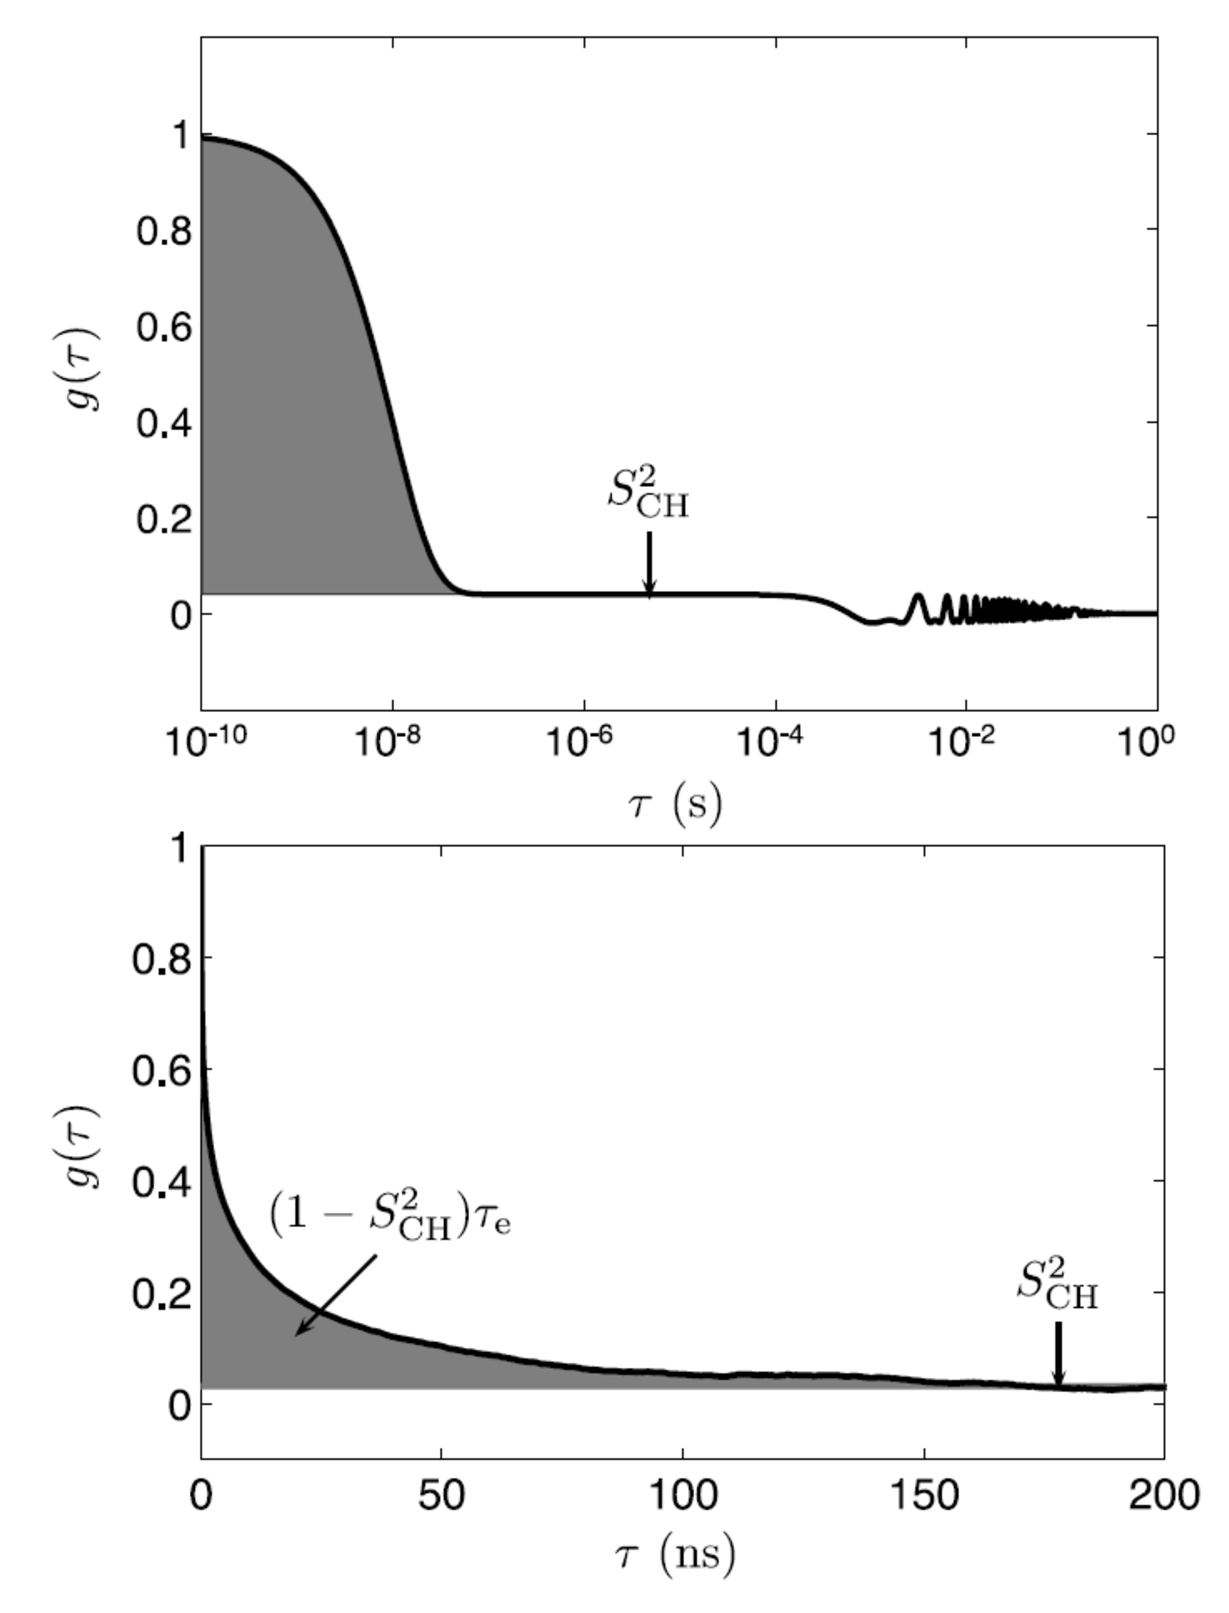
\includegraphics[width=8.6cm]{../Fig/correlationF.eps}
\newline
  \caption{\label{correlationF}
    (Top) Illustration of the auto-correlation function g(τ) and effective
correlation time τe for a C–H bond in a lipid or surfactant bilayer. Magicangle
spinning with the frequency ωR leads to oscillations of g(τ) at the
frequencies ωR and 2ωR. The slow correlation time τs gives the final decay
of g(τ) towards zero. (Bottom) Example of g(τ) from a united-atom MD
simulation of a POPC bilayer in excess water, illustrating the decay towards
S2
CH. The effective correlation time τe is equal to the area in gray scaled by
(1 − S2
CH
)−1.
} 
\end{figure}

The rotational correlation function describes how long does it take for a single molecule
on average to sample the conformations. The effective correlation time 
\begin{equation}\label{effCTdef}
\tau_{e}:=\int_0^{\infty} \frac{g_{\rm{f}}(\tau)-S_{\rm{CH}}^2}{1-S_{\rm{CH}}^2} \mathrm{d}\tau
\end{equation} 
can be used as an intuitively useful single parameter to describe this time. 
The larger this parameter is, the longer it takes in average to sample the conformations related to the
bond. With this definition the area between the correlation function and its pleateau becomes $(1-S_{\rm{CH}}^2)\tau_{e}$.

\subsection{Detecting C--H bond dynamics experimentally}

The most used parameter to detect the C--H bond dynamics experimentally in time scales comparable to simulations
are the spin-lattice relaxation rates $R_1$ from deuterium labels and $^{13}$C. 
$R_1^{C}$ measured from $^{13}$C is connected to the spectral density (Eq.~\ref{FT}) through the equation
\begin{equation}\label{R1C}
R_{1}^{C}=\frac{D_{\rm{max}}^2N_{\rm{H}}}{20}\bigg[j(\omega_{\rm{H}}-\omega_{\rm{C}})+3j(\omega_{\rm{C}})+6j(\omega_{\rm{C}}+\omega_{\rm{H}})\bigg],
\end{equation}
where $\omega_{\rm{C}}$ and $\omega_{\rm{H}}$ are the Larmor angular frequencies of $^{13}$C and $^1$H respectively, 
$N_{\rm{H}}$ is the number of bound protons and $\frac{D_{\rm{max}}}{2\pi}\approx$22 kHz as in section~\ref{??}.
%is given by
%\begin{equation}
%d_{\rm{CH}}=-\frac{\mu_0\hbar\gamma_{\rm{H}}\gamma_{\rm{C}}}{4\pi\langle r_{\rm{CH}}^3\rangle},\nonumber
%\end{equation}
%where $\mu_0$ is the magnetic constant or vacuum permeability, $\hbar$ is the reduced Planck constant, 
%$\gamma_{\rm{C}}$ and $\gamma_{\rm{H}}$ are the gyromagnetic constants of $^{13}$C and $^1$H, respectively, 
%and $\langle r_{\rm{CH}}^3\rangle$ is the average cubic length of the C--H chemical bond. $d_{\rm{CH}}/2\pi$ is 
%approximately equal to -22 kHz for a methylene C--H bond \cite{Bec05:23285,Dvi05:607}.
$R_1^{D}$ measured from $^2$H is connected to the spectral density (Eq.~\ref{FT}) through the equation
\begin{equation}\label{R1C}
R_{1}^{D}=\frac{12\pi^2}{40}\bigg(\frac{e^2qQ}{h}\bigg)^2\bigg[j(\omega_{\rm{D}})+4j(2\omega_{\rm{D}})\bigg],
\end{equation}
where $\frac{e^2qQ}{h}$=170kHz as in the case of order parameters in section~\ref{??}.

Also the model free approach to measure the effective correlation time (Eq.~\ref{effCTdef}) was recently
introduced~\cite{ferreira15}. The method is based on the combination of experimental order parameter $S_{{\rm CH}}$,
spin-lattice relaxation rates $R_1$ and the transverse magnetization under a spin lock pulse $R_{1\rho}$ with measured 
appropriate nutation frequency.

%, defines the equilibration of $^{13}$C transverse magnetization under a spin lock pulse and is normally approximated as~\cite{Har86:NMRS}
%\begin{multline}\label{R1rho}
%R_{1\rho}(\omega_1)=\frac{d_{\rm{CH}}^2N_{\rm{H}}}{40}\bigg[4j(\omega_1)+j(\omega_{\rm{H}}-\omega_{\rm{C}})
%\\
%+3j(\omega_{\rm{C}})+6j(\omega_{\rm{H}})+6j(\omega_{\rm{C}}+\omega_{\rm{H}})\bigg],
%\end{multline}
%where $\omega_1$ is the nutation

%are spin
%lattice relaxation rates $R_1$ and $R_{1\rho}$

\subsection{Analyzing C--H bond dynamics from simulations}

As in the case of order parameters, the auto--correlation function for each C--H bond can be
calculated directly from simulations using the definition in Eq.~\ref{??} since the trajectories of each atom is known
as a function of time. As in the case of order parameters the positions of hydrogens can be determined 
for united atom models based on heavy atom positions and assuming tetrahedral configurations.
Usually in the correlation function calculation all the available time intervals from the 
simulation data are used and the average over those and all molecules is taken. However, since the 
amount of data decreases when the the time interval approaches the total length of the simulation,
usually the largest time interval used is the half of the total simulation length, for more details
see~\ref{gromacsMANUAL}.

To calculate the experimentally measurable spin lattice relaxation times, the spectral density (Eq.~\ref{FT})
must be first calculated. In principle, this could be done using numerical fourier transformations techniques, 
however this often leads to unneccessarily large fluctuations. Instead, commonly used apporach is to fit 
analytical functional form to the calculated auto--correlation function and then use analytical Fourier
transform of the fitted function. Most commonly the sum of ? or more exponentials is used as a fitting function but
also streched exponential has been used. Numerically the functional form of the fitting function should not matter as
long as the fit is good, however, theoretically the correct correlation function form to describe the modes of
physical motion can be debated. It is clear from correlation functions from simulations that one exponential 
is not enought to produce a good fit while ? gives a reasonable fit. This is not surprising since more
than one relaxation timescale is definitiely expected to be present in lipids in bilayer.

After the fitting the analytical form of the spectral density predicted by simulations is available.
Then its values can be calculated at the required larmor frequency values and substituted to Eqs.~\ref{R1C}
and~\ref{R1D} to get the $R_{1}^{C}$ and $R_{1}^{D}$. The value of the effective correlation time can be
calculated directly from the interated area below the correlation function, see Fig.~\ref{??} or from 
Eq. ??.




\subsection{Interplay between simulations and NMR spin lattice relaxation times: Validation and interpretation of dynamics}

The experimentally observable spin lattice relaxation parameter mentioned above ($R_1^{C}$, $R_1^{D}$ and $R_{1\rho}$)
are connected to the actual molecular dynamics through the spectral density (Eq.~\ref{FT}) which is the Fourier transformation
of the auto-correlation function~\ref{gt}. The spin lattice relaxation rates depends spectral density values only 
with certain larmor frequecies as seen from Eqs.~\ref{R1C} and~\ref{R1D}. In experiments the Larmor frequency 
depends on the external magnetic field of the used spectrometer. Thus, with a regular NMR spectrometer only
a single~\ref{R1C} and~\ref{R1D} values can be measured. These will only give information about the size
of the spectral density close to the used Larmor frequencies. However, to detect the whole rotational
correlation function one should have information with all relevant larmor frequency values. 
The single spin lattice relaxation rates only give an estimate how much of the dynamical prosesses
are present with the timescales roughly with inverse of Larmor frequency. Even the qualitative
changes in dynamics are difficult to detect by measuring single relaxation rate values since the
increase (decrease) of the value only indicates the increase (decrease) of relative significance 
of the relaxation with the detected timescales. If the general dynamics gets slower or faster depends
what happens to the significance of relaxation processes with faster and slower timescales which 
are not detected by measuring single relaxation rates.

Several experimental and theoretical apporaches has been use to address this issue.
Temperature dependence of spin relaxation rates have been measured to analyze the relative 
molecular rotational relaxation. 
Spectrometers with different magnetic field strenghts have been used to measure points with 
several Larmor frequencies.
Models are fitted to the spin relaxation data.
The effective correlation time is measured which gives a quantitative measure of the general 
rotational dynamics. Also MD simulations have been succesfull in interpretation of the 
measurements of the effect of double bonds on molecular dynamics. 

Comparison between spin lattice relaxation rates measured with NMR and calculated from MD
is also used to validate the correctness of the dynamics in the simulations.
The comparison in the early simulations revealed that there are dynamical
time scales present in simulations are realistic~\cite{??}. Later on the 
comparison between simulations and dispersion data indicated that the
simulation dynamics more or less agrees with experiments for some carbons
while there is room for improvement for others~\cite{??}. However, due to
the complicated connection between spin lattice relaxation rates and molecular dynamics
it is difficult to conclude from these comparison if the dynamics is too slow or
fast in the simulations. This issue can be clarified by measuring the effective correlation
times with recently introduced methods~\cite{ferrerira15}. The comparison between 
effective correlation times from experiments and simulations reveals that
the rotational correlation dynamics is too slow for the glycerol backbone and choline 
in Berger model. However, this is not very surprising since the Berger model is also sampling wrong configurations for
these segments. However, the experimental data and similar comparison would be useful
for models sampling more realistic strucutres, e.g. CHARMM36 which dynamics do not fully
satisfy the dispersion data.


\newpage
\onecolumngrid

\section{Stucture factors from scattering and simulations}

\noindent {\bf For this section I would be more than happy for some help} \\[0.1cm]

\noindent {\bf Here will be described:}\\[0.1cm]

\noindent How are the form factors are measured.\\
What is the primary experimental observable. \\

\noindent {\bf On these questions I do not know the answer and it is not exactly clear from where I can find the answers. More specifically:}  \\

\todo{Which is the experimental quantity that the scattering machinary exatcly puts out? \\
How the form factor is determined from the experimental observables? \\
Which assumptions are needed here? \\
There is already some discussion about this in the blog by Peter Heftberger and Georg Pabst, but any kind of information from full 
exaplanation with citations to the hints of relevant literature are helpful here.
The more detailed discussion can be found at:
{\tt https://github.com/NMRLipids/NMRLipids\_V-Review/issues/1}}

\vspace*{5mm}

\noindent How accurate are the experimental form factors. \\

\todo{Has this been discussed in the literature already?
Any kind of information from full exaplanation with citations to the hints of relevant literature are helpful here.
The more detailed discussion can be found at:
{\tt https://github.com/NMRLipids/NMRLipids\_V-Review/issues/2}}

\vspace*{5mm}

\noindent How the form factor is calculated from simulations and compared to experimental ones. \\

\todo{As far as I have understood, the form factor is simply a Fourier transform of electron density. I have some quick and dirty scripts to calculate those in the NMRLipids III repository: \\
{\tt https://github.com/NMRLipids/NmrLipidsCholXray/blob/master/scratch/FFactor/FFstructCALC.sh}\\
{\tt https://github.com/NMRLipids/NmrLipidsCholXray/tree/master/scratch/FFactor}\\
However, I have not been able to install the SIMtoEXP program ({\tt http://link.springer.com/article/10.1007\%2Fs00232-010-9254-5}) so I have not been able to check my script against the standard method.
This should be straighforward issue and should become clear once I check the details. Anyway, any kind of information from full exaplanation with citations to the hints of relevant literature are helpful here.
The more detailed discussion can be found at:
{\tt https://github.com/NMRLipids/NMRLipids\_V-Review/issues/3}}

\vspace*{5mm}

\noindent How accurate are the calculated form factors from simulations. \\

\todo{I think that from statistical point of view accuracy is quite high, however I am not sure about the effect of undulations etc.
Any kind of information from full exaplanation with citations to the hints of relevant literature are helpful here. 
The more detailed discussion can be found at:
{\tt https://github.com/NMRLipids/NMRLipids\_V-Review/issues/4}}

\vspace*{5mm}

\noindent What can be learned about the structure when comparing the form factors between experiments and simulations \\

\todo{I have thought that if the form factor is reproduced by the simulation, the electron density profile should be 
reasonable. However, since some people are tuning the peak highs for better agreement, I am not sure. 
There is also some connection to the thickness. There is already some discussion about this in the blog with
Peter Heftberger and Georg Pabst.
Any kind of information from full exaplanation with citations to the hints of relevant literature are helpful here.
The more detailed discussion can be found at:
{\tt https://github.com/NMRLipids/NMRLipids\_V-Review/issues/5}}



\section{Conclusions}

% Tables may be be put in the text as floats.
% Here is an example of the general form of a table:
% Fill in the caption in the braces of the \caption{} command. Put the label
% that you will use with \ref{} command in the braces of the \label{} command.
% Insert the column specifiers (l, r, c, d, etc.) in the empty braces of the
% \begin{tabular}{} command.
%
% \begin{table}
% \caption{\label{} }
% \begin{tabular}{}
% \end{tabular}
% \end{table}

% If you have acknowledgments, this puts in the proper section head.
\begin{acknowledgments}
% Put your acknowledgments here.
\end{acknowledgments}

% Create the reference section using BibTe
\bibliography{refs.bib}

%\newpage
%\section{APPENDIX: The NMR results reported by Tiago Ferreira}

\listoftodos

\end{document}
%
% ****** End of file aiptemplate.tex ******
